% --- Grounding DINO and DINOv2 ---
% --- Detection: Grounding DINO ---
\begin{frame}{Detection Foundation Model: Grounding DINO}
  \begin{itemize}
    \item Open-vocabulary detection with natural-language grounding.
    \item Uses transformer-based backbone for both image and text encoding.
    \item Matches object proposals in an image with user-provided text prompts (e.g.\ ``a red backpack'').
    \item Produces bounding boxes, labels, and confidence scores for detected objects.
    \item \textbf{Key architectural mechanisms}:
      \begin{itemize}
        \item \textbf{Feature enhancer neck} with deep image--text cross-attention (not only late fusion).
        \item \textbf{Language-guided query selection} to initialize decoder queries on relevant regions.
        \item \textbf{Cross-modality decoder head} for iterative region-text refinement.
      \end{itemize}
    \item \textbf{Result:} strong transfer to unseen categories and prompts; the text encoder builds on the CLIP-style grounding idea from the previous section.
  \end{itemize}
\end{frame}

\begin{frame}{Grounding DINO: How It Works}
  \centering
  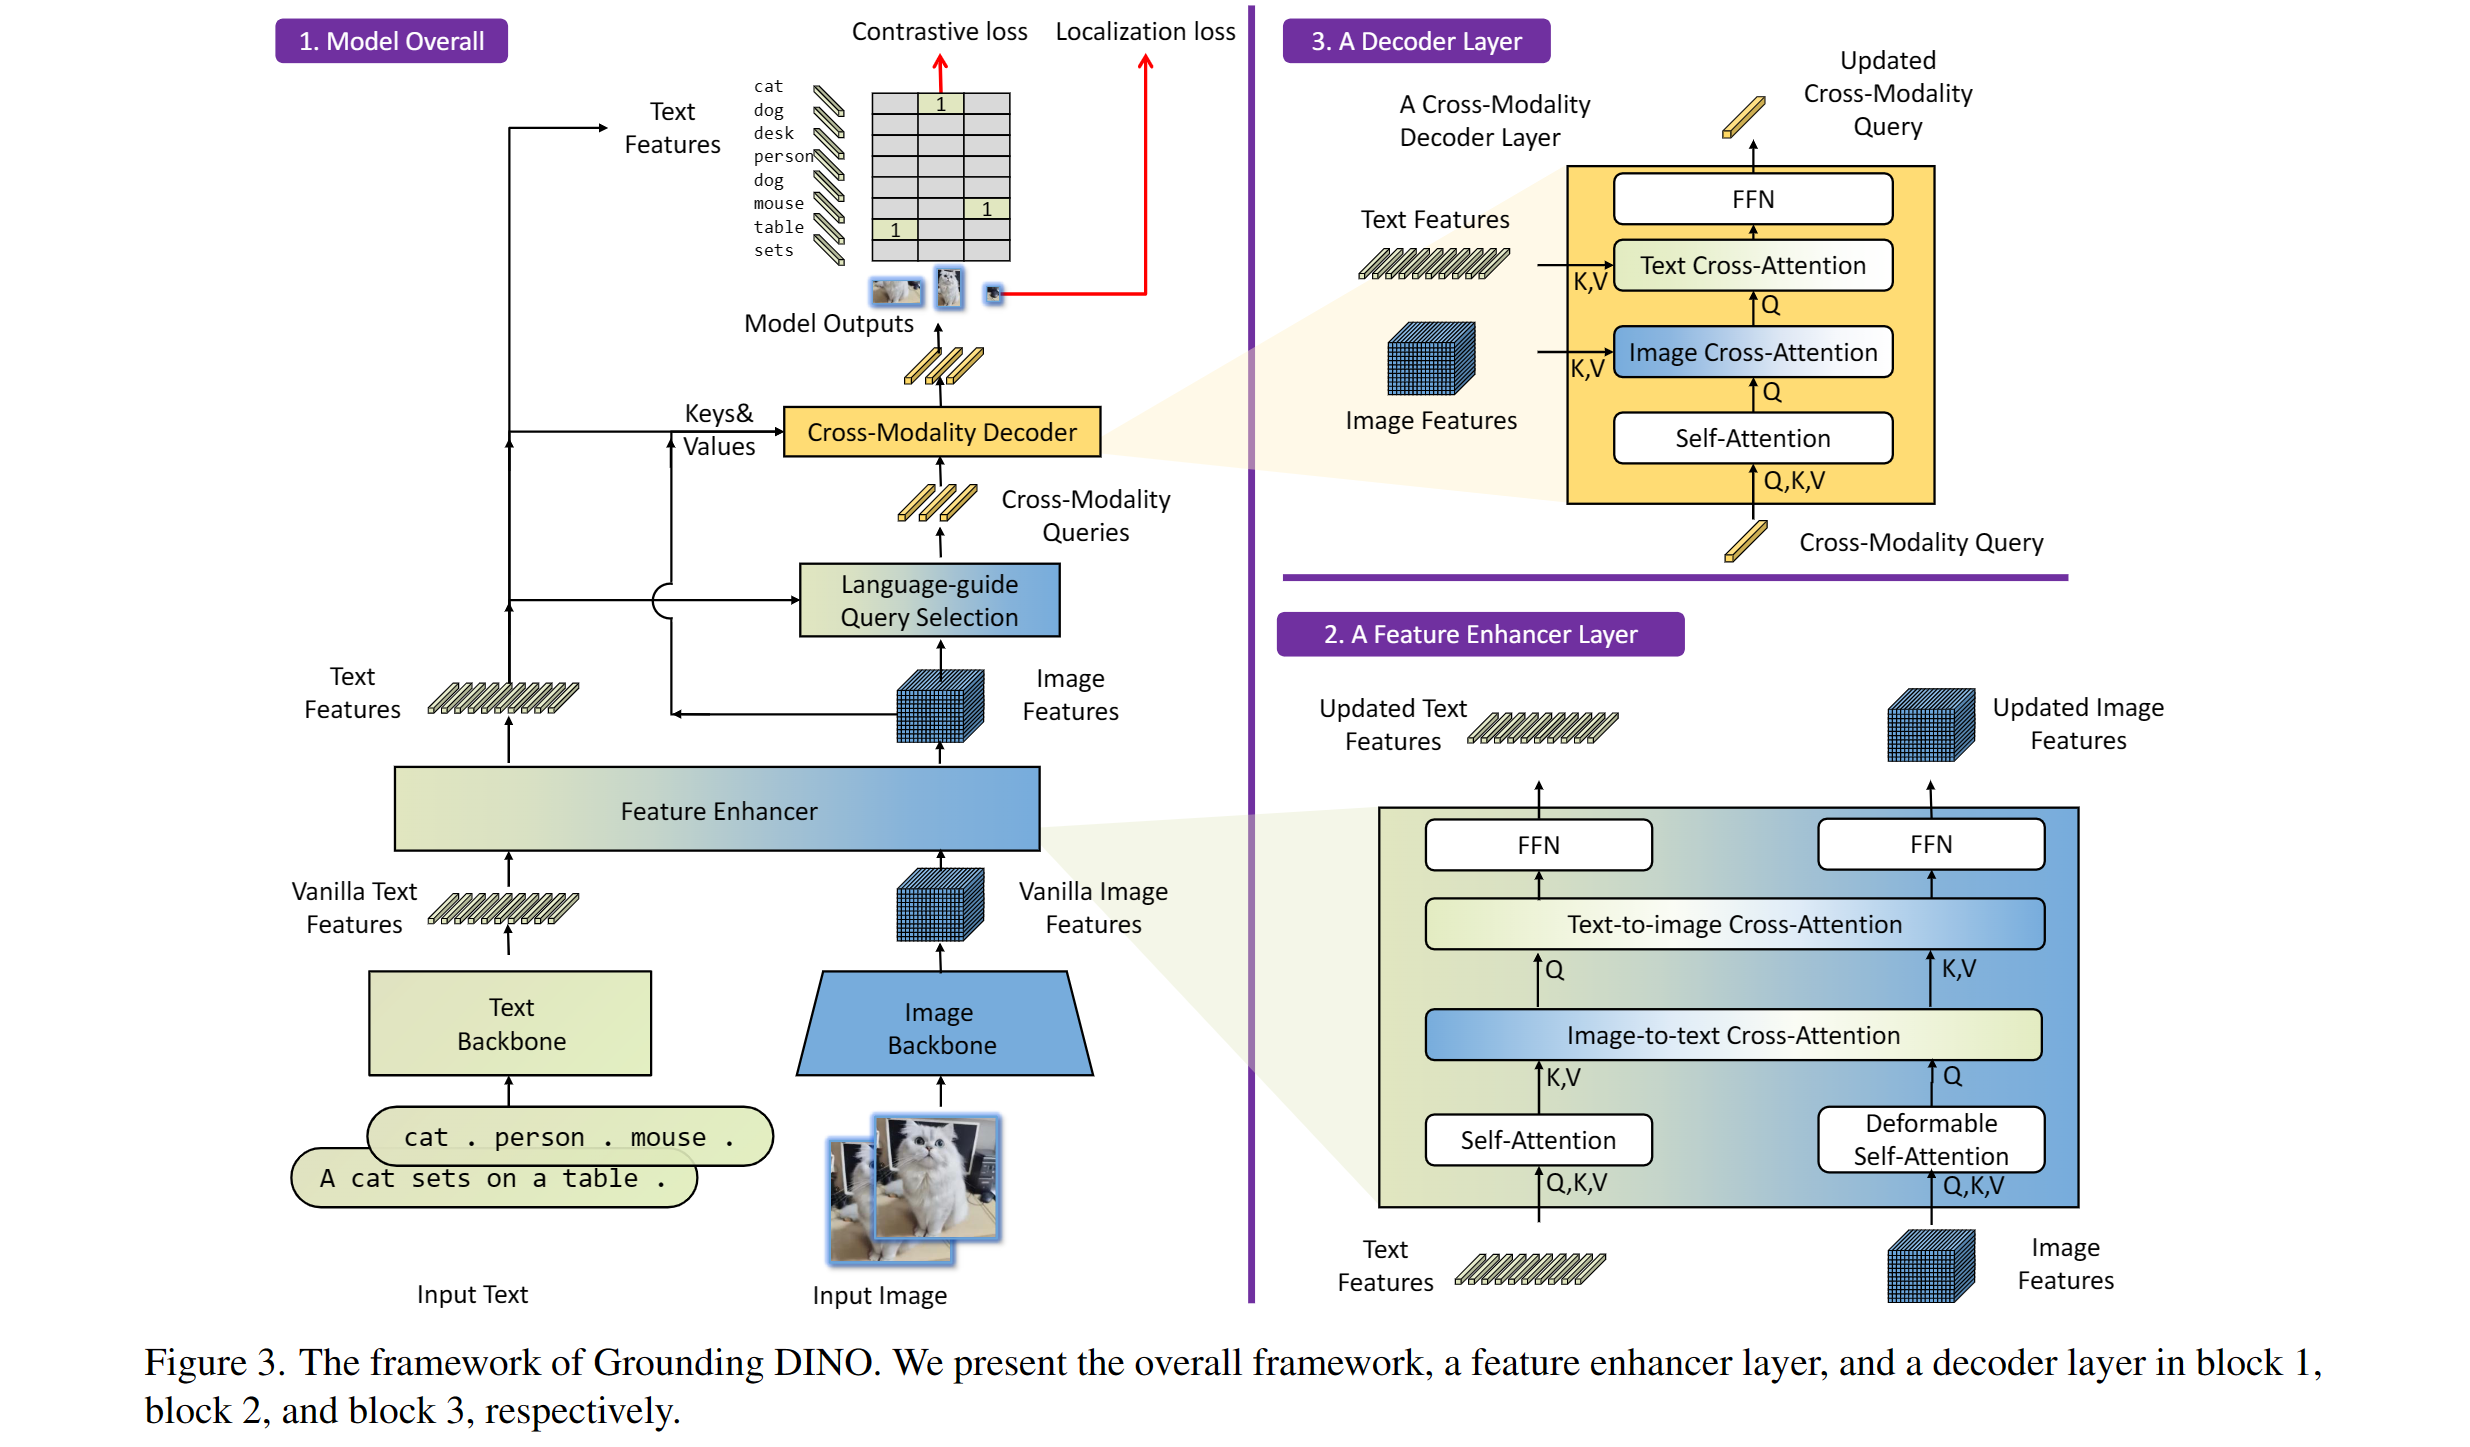
\includegraphics[width=0.8\textwidth]{images/foundation-models/grounding_dino_example.png}
\end{frame}

\begin{frame}{DINOv2: A Vision-Only Foundation Backbone}
  \begin{itemize}\itemsep0.28em
    \item Scales the \textbf{self-distillation} recipe from the contrastive-methods lecture (DINO image-level loss + iBOT masked-token loss) into a foundation model.
    \item \textbf{Curated data instead of raw web data:} LVD-142M is built by retrieving images similar to curated seed datasets from a large web pool, with deduplication. Data curation is a core part of the recipe.
    \item Train a large ViT ($\sim$1.1B parameters), then \textbf{distill} it into smaller ViTs for deployment.
    \item \textbf{Frozen features} transfer to classification, segmentation, depth, and retrieval without fine-tuning; Depth Anything (later this lecture) uses a DINOv2 encoder.
    \item \textbf{DINOv3} (2025) scales further (7B-parameter ViT) and adds a gram-anchoring loss to keep \textbf{dense} patch features clean at long training schedules.
  \end{itemize}
\end{frame}

\begin{frame}{DINOv2: Self-Supervised Training at Scale}
  \centering
  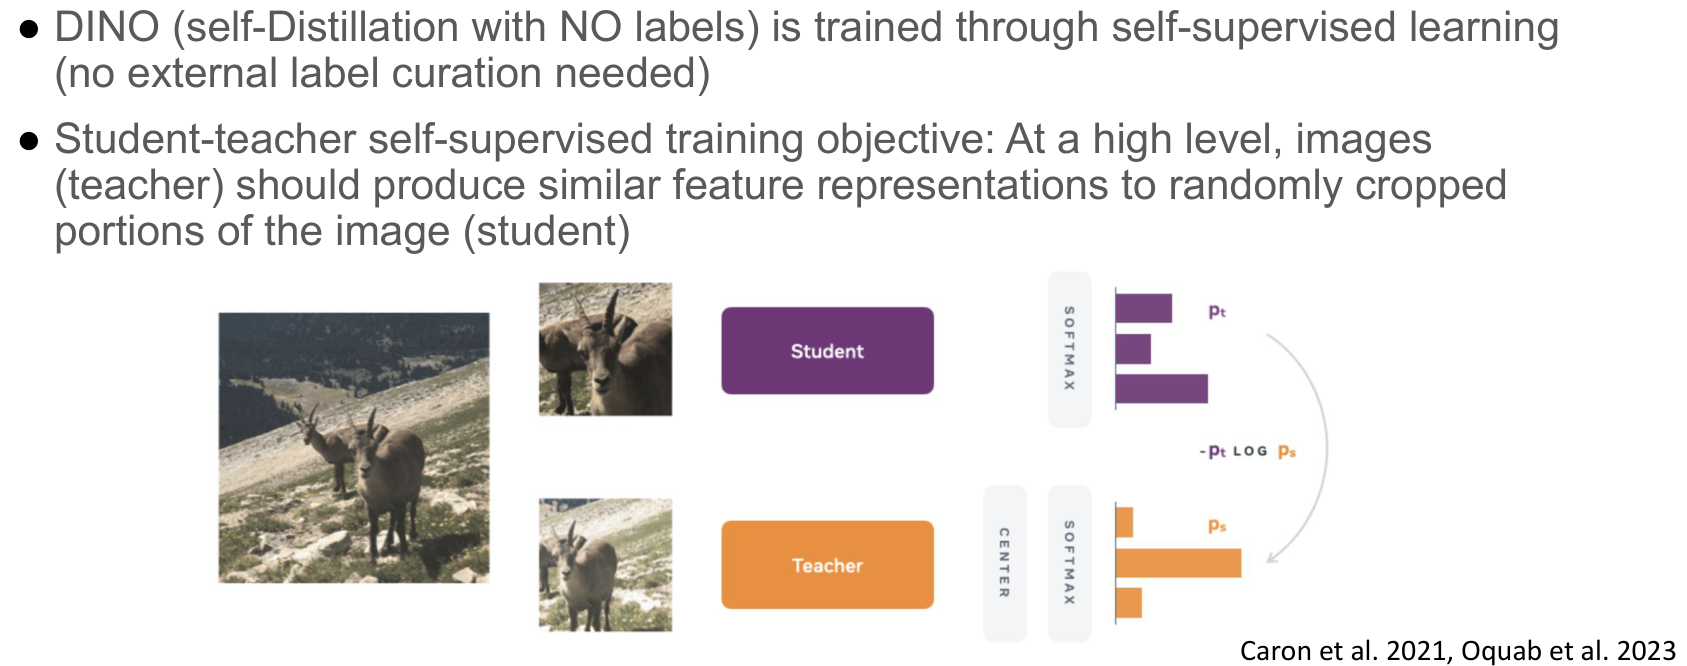
\includegraphics[width=\textwidth,height=0.86\textheight,keepaspectratio]{images/foundation-models/dino_self_supervised_training.png}
\end{frame}

\begin{frame}{DINOv2: One Frozen Backbone, Many Downstream Tasks}
  \centering
  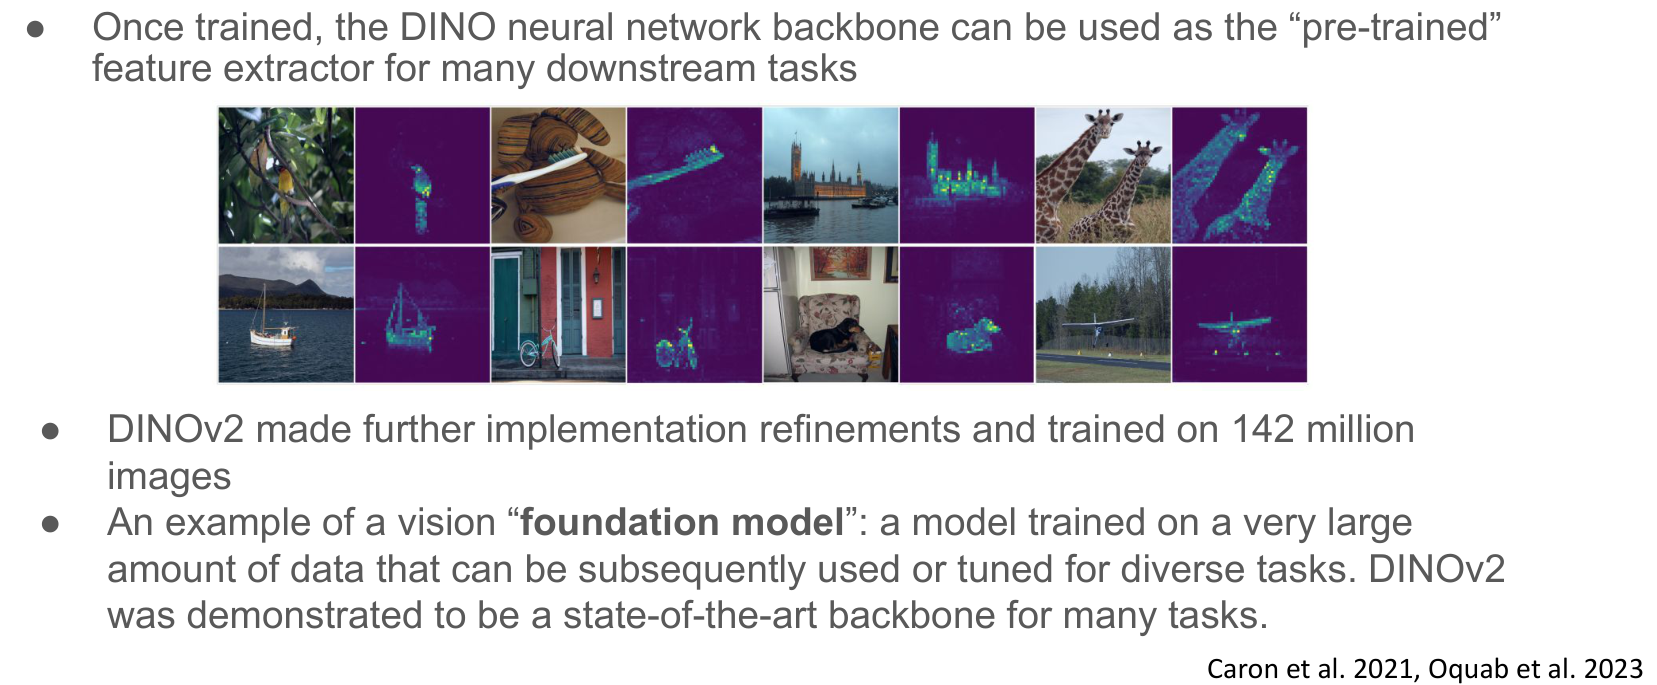
\includegraphics[width=\textwidth,height=0.86\textheight,keepaspectratio]{images/foundation-models/dinov2_backbone_downstream_tasks.png}
\end{frame}
